\documentclass[11pt,compress,t,notes=noshow, aspectratio=169, xcolor=table]{beamer}

\usepackage{../../style/lmu-lecture}
% Defines macros and environments
% This file is included in slides and exercises

% Rarely used fontstyle for R packages, used only in 
% - forests/slides-forests-benchmark.tex
% - exercises/single-exercises/methods_l_1.Rnw
% - slides/cart/attic/slides_extra_trees.Rnw
\newcommand{\pkg}[1]{{\fontseries{b}\selectfont #1}}

% Spacing helpers, used often (mostly in exercises for \dlz)
\newcommand{\lz}{\vspace{0.5cm}} % vertical space (used often in slides)
\newcommand{\dlz}{\vspace{1cm}}  % double vertical space (used often in exercises, never in slides)
\newcommand{\oneliner}[1] % Oneliner for important statements, used e.g. in iml, algods
{\begin{block}{}\begin{center}\begin{Large}#1\end{Large}\end{center}\end{block}}

% Don't know if this is used or needed, remove?
% textcolor that works in mathmode
% https://tex.stackexchange.com/a/261480
% Used e.g. in forests/slides-forests-bagging.tex
% [...] \textcolor{blue}{\tfrac{1}{M}\sum^M_{m} [...]
% \makeatletter
% \renewcommand*{\@textcolor}[3]{%
%   \protect\leavevmode
%   \begingroup
%     \color#1{#2}#3%
%   \endgroup
% }
% \makeatother


\newcommand{\pih}{\fh}
\newcommand{\gh}{\hat{g}}

\title{Interpretable Machine Learning}
% \author{LMU}
%\institute{\href{https://compstat-lmu.github.io/lecture_iml/}{compstat-lmu.github.io/lecture\_iml}}
\date{}

\begin{document}

	
% Set style/preamble.Rnw as parent.

% Load all R packages and set up knitr

% This file loads R packages, configures knitr options and sets preamble.Rnw as 
% parent file
% IF YOU MODIFY THIS, PLZ ALSO MODIFY setup.Rmd ACCORDINGLY...

% Defines macros and environments

\newcommand{\titlefigure}{figure/lime_credit_ice2.pdf}
\newcommand{\learninggoals}{
    \item See real-world data examples
    \item See application to image and text data}

\lecturechapter{LIME Examples}
\lecture{Interpretable Machine Learning}

% Prerequisite: le-intro

% ------------------------------------------------------------------------------

\begin{frame}[c]{Example on Credit Dataset (Tabular)}
	\begin{itemize}
		\item Model: SVM with RBF kernel
		\item $\xv$: first data point of the dataset with $\fh_{bad}(\xv) = 0.658$
		\item $\zv$: training data $\leadsto$ weighted by the Gower proximity 
		\item Surrogate model $\gh$: L$_1$-regularized linear model with 5 features 
	\end{itemize}

    \bigskip

	\begin{table}[ht]
		\centering
		\scriptsize
		\begin{tabular}{rlrlllrrl}
			\hline
			age & sex & job & housing & saving & checking & credit.amount & duration & purpose \\ 
			\hline
			 22 & female &   2 & own & little & moderate & 5951 &  48 & radio/TV \\ 
			\hline
		\end{tabular}
	\end{table}

\end{frame}

\begin{frame}[c]{Example on Credit Dataset (cont'd)}


\begin{center}
	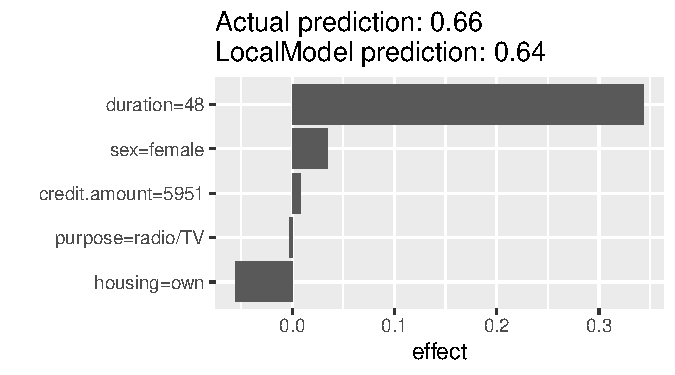
\includegraphics[width=0.45\textwidth]{figure/lime_credit.pdf}\\
	{Effects of surrogate model, i.e. $\thetah^T \xv$}
\end{center}

\begin{itemize}
	\item The local model prediction for $\xv$ is $\gh(\xv) = 0.64$ vs. $\fh(\xv) = 0.658$ 
	\item $\gh$ has a local fidelity of $L(\pih, \gh, \neigh) = 4.82$ with $\neigh(\zv)$ as the Gower proximity and $L(\pih_{bad}(\zv), g(\zv))$ as the euclidean distance 
\end{itemize}

\end{frame}
	
\begin{frame}[c]{Example on Credit Dataset (cont'd)}

\begin{itemize}	
	\item 2-dim ICE plots (aka. prediction surface plot) of credit amount and duration show how the surrogate model $g$ linearly approximates the previously nonlinear prediction surface of $\pih_{bad}$ 
\end{itemize}
\vspace{-0.4cm}
 \begin{columns}[totalwidth=\textwidth]
	\begin{column}{0.47\textwidth}
		\begin{center}
		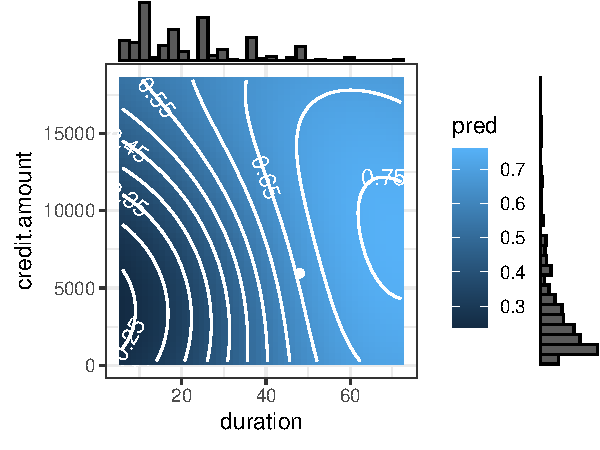
\includegraphics[width=1\textwidth]{figure/lime_credit_ice1.pdf}
		\end{center}		
	\end{column}
	\begin{column}{0.46\textwidth}  
		\begin{center}
				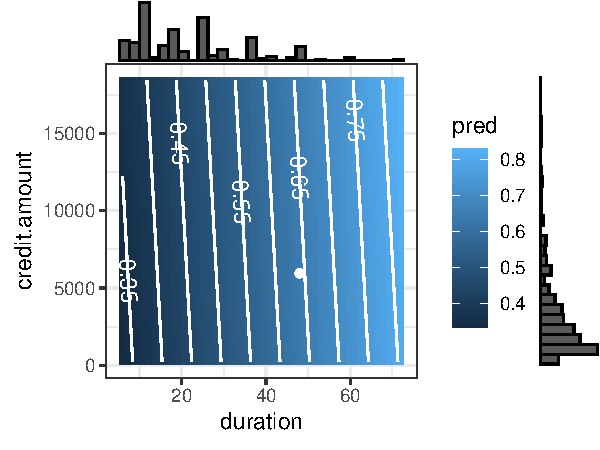
\includegraphics[width=1\textwidth]{figure/lime_credit_ice2.pdf}
		\end{center}
			
	\end{column}
\end{columns}
\vspace{-0.4cm}
\begin{center}
		{2-dim ICE plot of $\fh_{bad}$ (\textbf{left}) and surrogate $g$ (\textbf{right}) for features duration and credit amount. \\The white dot is $\xv$. The histograms display the marginal distribution of the training data $\Xmat$.}
\end{center}

\end{frame}

%\begin{frame}[containsverbatim,allowframebreaks]{Bike Sharing Dataset}
%\vspace{-.3cm}
%
%\begin{center}
%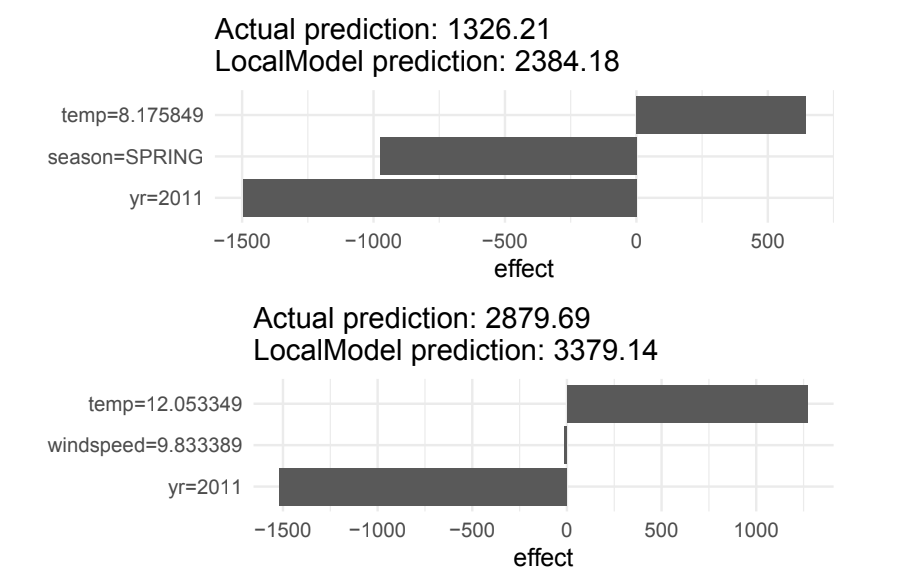
\includegraphics[width=0.7\textwidth]{figure/bike-figure.png}
%\end{center} 
%
%\footnotesize \textbf{Figure:} LIME for two example instances of the bike sharing dataset.
%
%\normalsize
%\vspace{0.2cm}
%The plots show the feature effect of the sparse linear model, i.e. the model coefficients times the feature value of the instance.
%Warmer temperature has a positive effect on the prediction, 
%while the year 2011 has a large negative effect as well as the springtime.
%\end{frame}

\begin{frame}{LIME for Text Data \citebutton{Shen, Ian, (2019)}{https://medium.com/just-another-data-scientist/explain-sentiment-prediction-with-lime-f90ae83da2da}}
    LIME can also be applied to text data: 
	\begin{itemize}
		\item Raw text representations: 
		\begin{itemize}
		    \item Binary vector indicating the presence or absence of a word 
		    \item A vector of word counts
		\end{itemize}
		\item Examples for \textit{``This text is the first text."} and \textit{``Finally, this is the last one."}:
		\begin{center}
			\begin{tabular}{c|c|c|c|c|c|c|c} 
				this & text & is & the & first & finally & last & one \\ 
				\hline
				1 & 2 & 1 & 1 & 1 & 0 & 0 & 0 \\
				1 & 0 & 1 & 1 & 0 & 1 & 1 & 1 \\
			\end{tabular}
		\end{center} 
		\item \textbf{Sampling}: Randomly set the entry of individual words to $0$; equal to removing all occurrences of this word in the text. 
		\item \textbf{Proximity}: Exponential kernel with cosine distance. 
		\begin{itemize}
		    \item Neglects words that do not occur in both texts 
		    \item Measures the distance irrespective of the text size
		\end{itemize}
	\end{itemize}
\end{frame}
	
\begin{frame}{LIME for Text Data (cont'd) \citebutton{Shen, Ian, (2019)}{https://medium.com/just-another-data-scientist/explain-sentiment-prediction-with-lime-f90ae83da2da}}	 
	\begin{itemize}
		\item Random forest classifier labeling movie reviews from IMDB 
		\begin{itemize}
		    \item \textcolor{blue}{0}: negative
		    \item \textcolor{orange}{1}: positive
		\end{itemize}
		\item Surrogate model is a sparse linear model 
	\end{itemize}
	
	\begin{figure}
		\begin{center}
			%\captionsetup{font = scriptsize, labelfont = {bf, scriptsize}}
			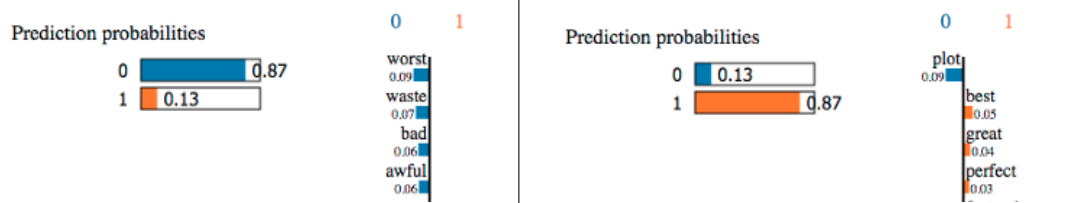
\includegraphics[width=0.9\textwidth]{figure/lime_movier}
		\end{center}
	\end{figure}
	
	{Words like ``worst`` or ``waste`` indicate negative review while words like ``best`` or ``great`` indicate positive review}
	
	\end{frame}
	
\begin{frame}[c]{LIME for image data}
	\begin{columns}[totalwidth=\textwidth]
		\begin{column}{0.67\textwidth}
			LIME also works for image data:  
			\begin{itemize}
				\item \textbf{Idea}: Each obs. is represented by a binary vector indicating the presence or absence of superpixels \citebutton{Achanta et al. 2012}{https://ieeexplore.ieee.org/document/6205760}
				\item Superpixels are interconnected pixels with similar colors (absence of a single pixel might not have a (strong) effect on the prediction)
				\item \textbf{Warning}: Size of superpixels needs to be determined before the segmentation takes place
				\item \textbf{Sampling}: Randomly switching some of the super pixels ``off", i.e., by coloring some superpixels uniformly
			\end{itemize}		
		\end{column}
		\begin{column}{0.26\textwidth}  
			\begin{center}
				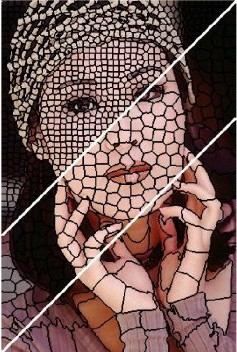
\includegraphics[width=1\textwidth]{figure/superpixel_woman}
				{Example for superpixels of different sizes}
			\end{center}
		\end{column}
	\end{columns}
    
\end{frame}
\begin{frame}{LIME for image data (cont'd) \citebutton{Ribeiro. 2016}{https://github.com/marcotcr/lime}}
	\begin{itemize}
		\item Explaining prediction of pre-trained inception neural network classifier
		\item \textbf{Sampling}: Graying out all superpixels besides 10 superpixels
		\item \textbf{Surrogate}: Locally weighted sparse linear models 
		\item \textbf{Proximity}: Exponential kernel with euclidean distance
	\end{itemize}
% https://lime-ml.readthedocs.io/en/latest/lime.html#module-lime.lime_image
	\vspace{-0.3cm}
	\begin{center}
		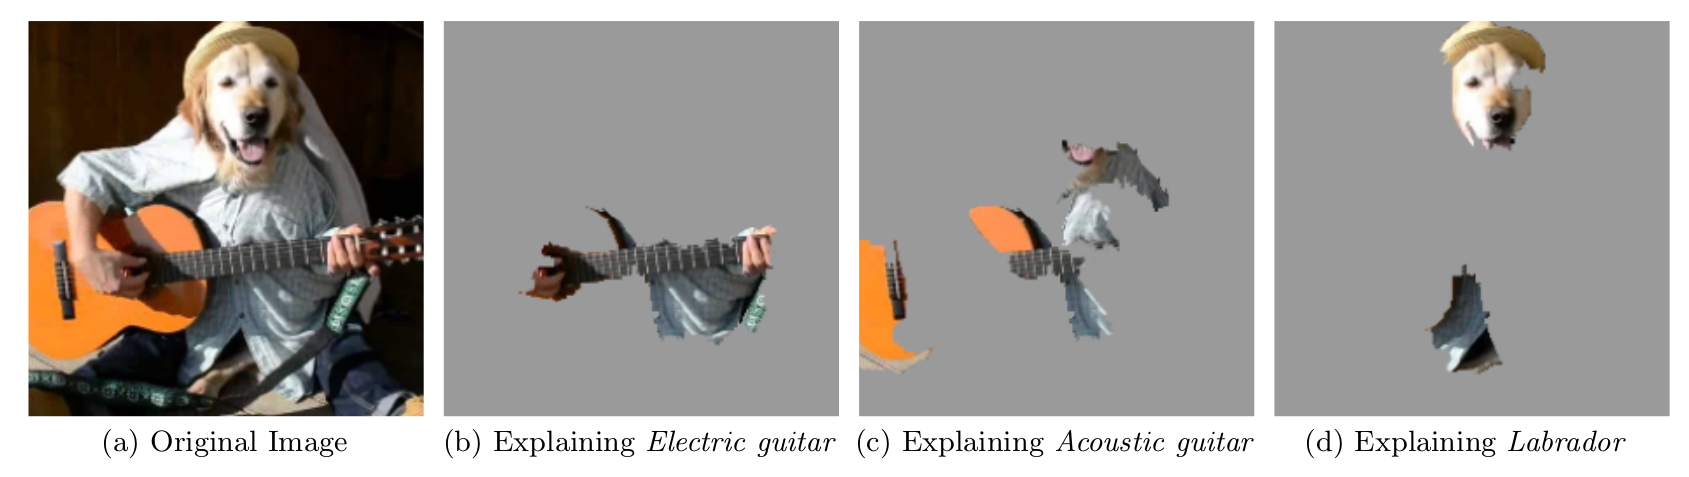
\includegraphics[width=0.8\textwidth]{figure/lime-images}
		
		{Top 3 classes predicted}
	\end{center}
	
\end{frame}
\endlecture
\end{document}
